\documentclass[12pt, a4paper]{scrreprt}
\usepackage[utf8]{inputenc}
\usepackage[ngerman]{babel}
\usepackage[bookmarksnumbered]{hyperref}
\usepackage{graphicx}

\begin{document}
\begin{titlepage}
\titlehead{
	\begin{minipage}[c][5cm][c]{5cm}
	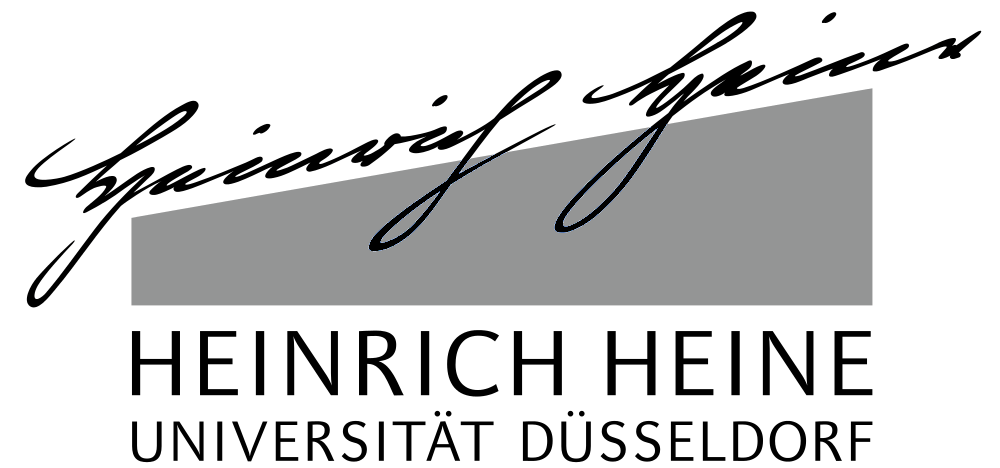
\includegraphics[width=48mm]{logo2}
	\end{minipage}
	\hfill
	\begin{minipage}[c][5cm][c]{10cm}
	\begin{flushright}
	\textbf{Universität Düsseldorf\\Mathematisch-Naturwissenschaftliche Fakultät\\Institut für Informatik\\Dozent:} PD Dr. Wilfried Linder
	\end{flushright}
	\end{minipage}
}
\subject{Benutzerhandbuch}
\title{Dungeon Crawler 	
	\begin{minipage}[c][1cm][c]{1cm}
	
\includegraphics[width=10mm]{Icon}
	\end{minipage}}
\subtitle{Programmierpraktikum im Sommersemester 2013}
\author{Michael Beurskens\\ Robin Thüs\\ Ruslan Curbanov}
\publishers{Gruppe 22}
\maketitle
\end{titlepage}
\tableofcontents
\chapter{Einleitung}
\section{Vorwort und Systemanforderungen}
\section{Befehlsliste und Steuerung}
\section{Prolog}
\section{Besetzung}
\section{Schauplätze}
\chapter{Einrichten des Spiels}
\section{Hauptmenü}
\begin{picture}(250,100)(50,50)
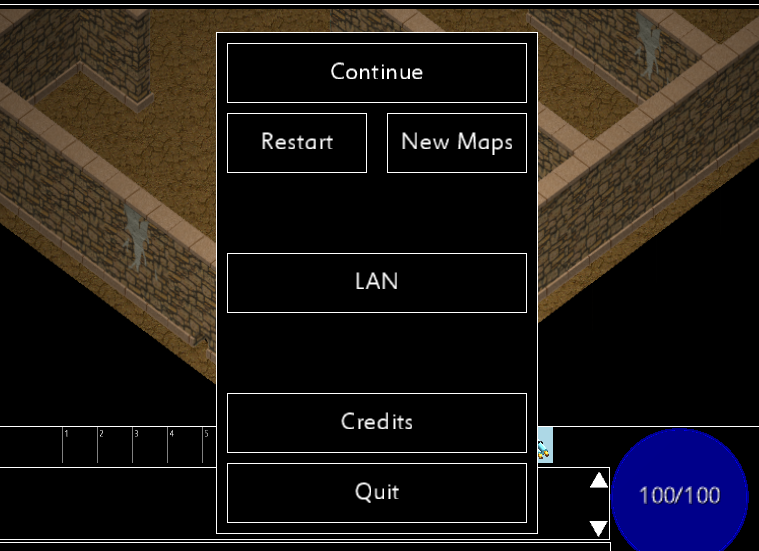
\includegraphics[width=\textwidth]{img/menu}
\end{picture}
\section{Optionen}
\chapter{Gameplay und Anzeigesysteme}
\chapter{Multiplayer}
\section{Die Lobby}
\section{Das Chatsystem}
\chapter{Speichern und Laden}
\chapter{Lizenzbedingungen}
\chapter{Support}
\end{document}